% =============================================================================
%  Relatório da AB2 de Computação Gráfica: sala de aula 3D navegável em OpenGL
%  Formatação: Manual para normalização de trabalhos acadêmicos da UFAL (SIBI, 2. ed., 2025),
%  sobre a classe abnTeX2. Compilar: latexmk -pdf relatorio.tex (veja README.md desta pasta).
% =============================================================================
\documentclass[
  12pt,          % fonte 12 no texto (manual UFAL, 3.2.1 b)
  oneside,       % documento digital, só anverso
  a4paper,       % A4 (21 x 29,7 cm)
  chapter=TITLE, % seção primária em caixa alta
  english,
  brazil,        % último idioma = idioma principal
]{abntex2}

% --- Pacotes ------------------------------------------------------------------
\usepackage[T1]{fontenc}
\usepackage[utf8]{inputenc}
\usepackage{newtxtext,newtxmath}  % Times (manual UFAL: Times New Roman ou Arial)
\usepackage{microtype}
\usepackage{graphicx}
\usepackage{subcaption}
\usepackage{amsmath}
\usepackage{tabularx}
\usepackage{xcolor}
\usepackage{listings}
\usepackage{tikz}
\usetikzlibrary{positioning,arrows.meta}
\usepackage{csquotes}
\usepackage[style=abnt,backend=biber]{biblatex}  % NBR 6023 e citação autor-data da NBR 10520:2023
\addbibresource{referencias.bib}

% --- Margens (manual UFAL, Figura 2): 3 cm superior e esquerda, 2 cm inferior e direita
\setlrmarginsandblock{3cm}{2cm}{*}
\setulmarginsandblock{3cm}{2cm}{*}
\checkandfixthelayout

% --- Títulos na mesma fonte do texto (manual UFAL, 3.4): primária em negrito e caixa alta,
%     secundária em negrito, terciária sem negrito; todos em 12
\renewcommand{\ABNTEXchapterfont}{\rmfamily\bfseries}
\renewcommand{\ABNTEXchapterfontsize}{\normalsize}
\renewcommand{\ABNTEXsectionfont}{\rmfamily\bfseries}
\renewcommand{\ABNTEXsectionfontsize}{\normalsize}
\renewcommand{\ABNTEXsubsectionfont}{\rmfamily\mdseries}
\renewcommand{\ABNTEXsubsectionfontsize}{\normalsize}

% --- Quadros (tabelas de texto) e códigos ---------------------------------------
% O babel redefine os nomes ao iniciar o documento: a troca vai para \captionsbrazil.
\addto\captionsbrazil{%
  \renewcommand{\tablename}{Quadro}%
  \renewcommand{\listtablename}{Lista de quadros}%
}
\renewcommand{\lstlistingname}{Código}
\renewcommand{\lstlistlistingname}{Lista de códigos}
\renewcommand{\tableautorefname}{Quadro}
\providecommand*{\lstlistingautorefname}{Código}
\newcommand{\fonteautores}{\fonte{Elaborado pelos autores (2026).}}
\newcommand{\fonteautoras}{\fonte{Elaborada pelos autores (2026).}}

\definecolor{codigocomentario}{rgb}{0.35,0.45,0.35}
\definecolor{codigopalavra}{rgb}{0.10,0.20,0.55}
\lstset{
  language=C++,
  basicstyle=\ttfamily\footnotesize,
  keywordstyle=\color{codigopalavra}\bfseries,
  commentstyle=\color{codigocomentario}\itshape,
  frame=single,
  framesep=4pt,
  xleftmargin=6pt,
  xrightmargin=6pt,
  breaklines=true,
  columns=fullflexible,
  keepspaces=true,
  showstringspaces=false,
  captionpos=t,
  aboveskip=6pt,
  belowskip=0pt,
}
\lstdefinelanguage{GLSL}[ANSI]{C}{
  morekeywords={vec2,vec3,vec4,mat3,mat4,sampler2D,uniform,in,out,texture,normalize,dot,max,length,any,lessThan,greaterThan},
}

% --- Dados do trabalho --------------------------------------------------------
\titulo{SALA DE AULA 3D NAVEGÁVEL EM OPENGL: relatório técnico do projeto da AB2 de Computação Gráfica}
\autor{ERASMO DA SILVA SÁ JUNIOR\\JOSÉ RIQUELME TEIXEIRA DA SILVA\\VICTOR ANDRÉ LOPES BRASILEIRO}
\local{Maceió--AL}
\data{2026}
% Sem \instituicao: a folha de rosto do manual não tem essa linha (a natureza já cita a UFAL); a capa a escreve.
\tipotrabalho{Relatório técnico}
\preambulo{Relatório técnico apresentado à disciplina de Computação Gráfica do Instituto de Computação da
Universidade Federal de Alagoas, como requisito parcial para a avaliação da AB2.}
\orientador[Professor:]{Marcelo Costa Oliveira}

\makeatletter
\hypersetup{
  pdftitle={Sala de aula 3D navegável em OpenGL},
  pdfauthor={Erasmo da Silva Sá Junior; José Riquelme Teixeira da Silva; Victor André Lopes Brasileiro},
  pdfsubject={Relatório técnico da AB2 de Computação Gráfica (IC/UFAL)},
  pdfkeywords={OpenGL}{computação gráfica}{transformações geométricas}{iluminação}{textura projetiva},
  colorlinks=true,
  linkcolor=black,
  citecolor=black,
  urlcolor=black,
  bookmarksdepth=4,
}
\makeatother

% Capa no modelo do manual (Figura 7): instituição no alto, autores, título no meio, local e ano embaixo.
\renewcommand{\imprimircapa}{%
  \begin{capa}%
    \center
    {\bfseries\large UNIVERSIDADE FEDERAL DE ALAGOAS\par INSTITUTO DE COMPUTAÇÃO\par}
    \vspace*{2.5cm}
    {\large \imprimirautor\par}
    \vfill
    \begin{center}
      \large\textbf{SALA DE AULA 3D NAVEGÁVEL EM OPENGL:} relatório técnico do projeto da AB2 de Computação
      Gráfica
    \end{center}
    \vfill
    {\large \MakeUppercase{\imprimirlocal}\par \imprimirdata\par}
    \vspace*{1cm}
  \end{capa}
}

\begin{document}

\selectlanguage{brazil}
\frenchspacing

% =============================================================================
%  Elementos pré-textuais
% =============================================================================
\pretextual

\imprimircapa
\imprimirfolhaderosto

\begin{resumo}
Este relatório descreve o projeto da AB2 de Computação Gráfica: uma sala de aula tridimensional navegável,
escrita em C++17 com OpenGL 3.3 no perfil core, GLFW, GLAD, GLM e stb\_image. A sala de 8 × 3 × 7 m reúne
carteiras, cadeiras, quadro, mesa do professor, luminárias com interruptor, ventilador de parede, projetor,
tela retrátil e lixeira, todos modelados no código a partir de primitivas e organizados num grafo de cena
hierárquico. A cena é iluminada pelo modelo de Blinn-Phong por fragmento, com luzes pontuais atenuadas, luz
direcional de preenchimento, materiais por peça e texturas. O usuário navega com câmera livre (teclado e
mouse), inspeciona cada objeto isoladamente e interage com a sala: liga e desliga as luzes, abre a tela
retrátil, liga o ventilador e o projetor e troca os slides. As três transformações pedidas na avaliação são
detalhadas com suas matrizes: a escala em Y com pivô no topo da lona da tela retrátil, a rotação das pás do
ventilador em torno do eixo do motor, integrada no tempo, e a projeção do slide por textura projetiva, em
que o projetor é tratado como uma segunda câmera. O projeto compila com CMake e g++ no Windows
(MinGW-w64) e no Linux, com as bibliotecas embutidas no repositório, e o build limpo foi verificado em três
sistemas.

\textbf{Palavras-chave}: computação gráfica; OpenGL; transformações geométricas; iluminação; textura projetiva.
\end{resumo}

\begin{resumo}[Abstract]
\begin{otherlanguage*}{english}
This report describes the second assessment (AB2) project of the Computer Graphics course: a navigable 3D
classroom written in C++17 with core-profile OpenGL 3.3, GLFW, GLAD, GLM and stb\_image. The
8 × 3 × 7 m room contains student desks, chairs, a whiteboard, a teacher's desk, ceiling lamps with a wall
switch, a wall fan, a projector, a retractable screen and a trash can, all modeled in code from primitives
and arranged in a hierarchical scene graph. The scene is lit with per-fragment Blinn-Phong shading,
attenuated point lights, a directional fill light, per-part materials and textures. The user moves a free
camera with keyboard and mouse, inspects each object in isolation and interacts with the room: switching
the lights, opening the screen, turning on the fan and the projector and changing slides. The three
transformations required by the assessment are detailed with their matrices: a Y scale pivoted at the top of
the screen canvas, the rotation of the fan blades around the motor axis integrated over time, and the slide
projection through projective texture mapping, which treats the projector as a second camera. The project
builds with CMake and g++ on Windows (MinGW-w64) and Linux with bundled libraries, and a clean build was
verified on three systems.

\textbf{Keywords}: computer graphics; OpenGL; geometric transformations; lighting; projective texture mapping.
\end{otherlanguage*}
\end{resumo}

\pdfbookmark[0]{\listfigurename}{lof}
\listoffigures*
\cleardoublepage

\pdfbookmark[0]{\listtablename}{lot}
\listoftables*
\cleardoublepage

\pdfbookmark[0]{\lstlistlistingname}{lol}
\begin{KeepFromToc}
\lstlistoflistings
\end{KeepFromToc}
\cleardoublepage

\pdfbookmark[0]{\contentsname}{toc}
\tableofcontents*
\cleardoublepage

% =============================================================================
%  Elementos textuais
% =============================================================================
\textual

\chapter{Introdução}

O objetivo do projeto é construir, com OpenGL moderno, uma sala de aula tridimensional que possa ser
percorrida e manipulada em tempo real. A avaliação pede objetos modelados pela equipe, iluminação, texturas,
câmera navegável e interações que exercitem transformações geométricas: uma escala, uma rotação e uma
projeção, cada uma ligada a um objeto da sala.

O resultado é um único executável que abre a janela mostrada na \autoref{fig:cena-inicial}. A sala tem
6 carteiras e 6 cadeiras, quadro branco, mesa do professor, quatro luminárias de teto com interruptor de
parede, ventilador de parede, projetor preso ao teto, tela retrátil e lixeira. Nenhum modelo foi importado:
toda a geometria é gerada no código, a partir de caixas, cilindros, planos e malhas montadas vértice a vértice.

\begin{figure}[htb]
  \centering
  \caption{Vista inicial da sala, com as luzes acesas}
  \label{fig:cena-inicial}
  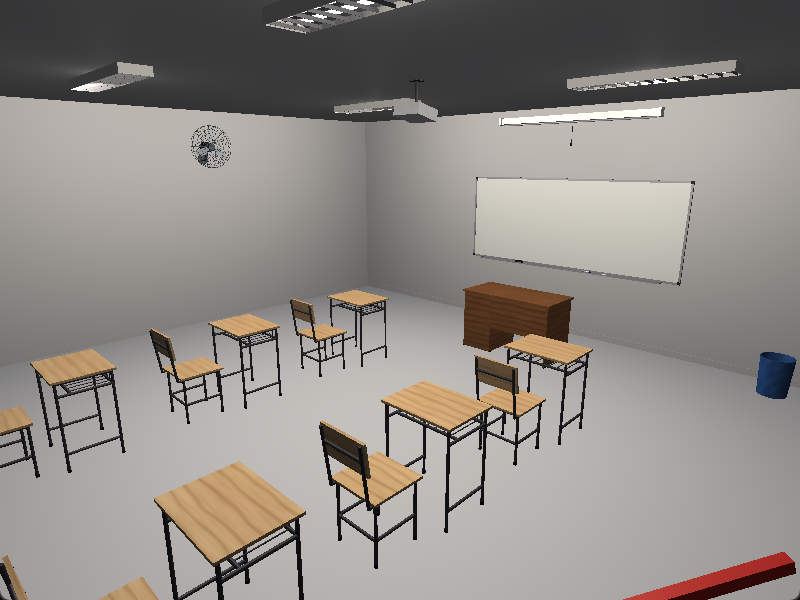
\includegraphics[width=0.85\textwidth]{figuras/cena-inicial.png}
  \fonteautoras
\end{figure}

As interações pedidas foram distribuídas assim: a tela retrátil usa a \textbf{escala} para abrir e recolher a
lona; o ventilador usa a \textbf{rotação} para girar as pás; e o projetor usa a \textbf{projeção} para lançar
o slide sobre a lona, o quadro ou a parede. Além delas, a sala tem luzes que acendem e apagam pelo interruptor.

O \autoref{cap:tecnologias} apresenta as tecnologias e o \autoref{cap:arquitetura}, a organização do código.
O \autoref{cap:modelagem} descreve a modelagem e a montagem da sala, e o \autoref{cap:transformacoes}
detalha as três transformações. O \autoref{cap:iluminacao} trata da iluminação, dos materiais e das texturas, e o
\autoref{cap:camera}, da câmera e da interação. Os resultados estão no \autoref{cap:resultados}; a compilação,
no \autoref{cap:compilacao}; a divisão de tarefas, no \autoref{cap:equipe}. O \autoref{cap:conclusao} conclui
o relatório. A lista completa de comandos está no Apêndice~\ref{ap:comandos}. O texto segue o manual de
normalização da UFAL \cite{ufal2025}.

% -----------------------------------------------------------------------------
\chapter{Tecnologias}
\label{cap:tecnologias}

O programa é escrito em C++17 e usa o OpenGL 3.3 no perfil \emph{core} \cite{segal2010}, que exige o
pipeline programável: não há \texttt{glBegin}/\texttt{glEnd} nem pilha de matrizes do pipeline fixo. Toda
geometria vai para a GPU em \emph{buffers} (VAO, VBO e EBO) e é desenhada por um par de shaders GLSL
(\texttt{shaders/basic.vert} e \texttt{shaders/basic.frag}). As matrizes são calculadas na CPU e enviadas
como \emph{uniforms}.

As bibliotecas de terceiros ficam no próprio repositório, em \texttt{lib/}, e são compiladas junto com o
projeto pelo CMake (\autoref{tab:bibliotecas}). Assim, o build não depende de pacotes instalados no sistema,
o que simplifica a compilação em máquinas diferentes.

\begin{table}[htb]
  \centering
  \caption{Bibliotecas usadas}
  \label{tab:bibliotecas}
  \small
  \begin{tabularx}{\textwidth}{|l|X|}
    \hline
    \textbf{Biblioteca} & \textbf{Uso no projeto} \\
    \hline
    GLFW 3.5.1 \cite{glfw} & Janela, contexto OpenGL, teclado, mouse e foco \\
    GLAD \cite{glad} & Carrega as funções do OpenGL 3.3 core fornecidas pelo driver \\
    GLM 1.0.3 \cite{glm} & Vetores, matrizes, \texttt{lookAt}, \texttt{perspective}, \texttt{rotate}, \texttt{scale} \\
    stb\_image \cite{stb} & Leitura das texturas PNG \\
    \hline
  \end{tabularx}
  \fonteautores
\end{table}

O build usa CMake com \emph{presets} (\texttt{CMakePresets.json}): \texttt{windows}, com o g++ do MinGW-w64
(MSYS2), e \texttt{linux}, com o g++ do sistema e os headers do X11. O \autoref{cap:compilacao} traz os passos.

% -----------------------------------------------------------------------------
\chapter{Arquitetura}
\label{cap:arquitetura}

O código é dividido em quatro camadas, com headers em \texttt{include/} e implementações em \texttt{src/}.
Cada camada só depende das que estão à sua direita na \autoref{fig:camadas}.

\begin{figure}[htb]
  \centering
  \caption{Camadas do código e sentido das dependências}
  \label{fig:camadas}
  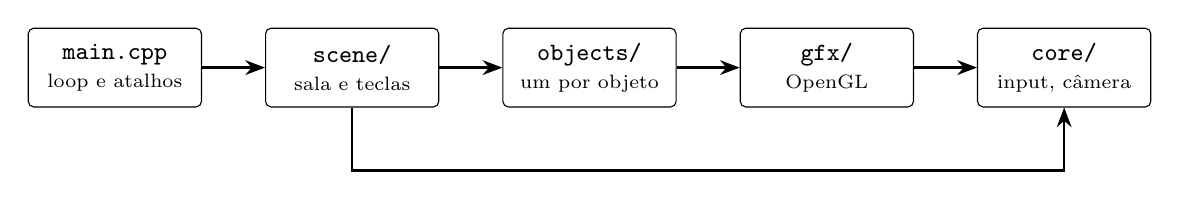
\begin{tikzpicture}[
      node distance=8mm,
      caixa/.style={draw, rounded corners=2pt, minimum width=22mm, minimum height=10mm, align=center, font=\small},
      seta/.style={-{Stealth[length=2.5mm]}, thick},
    ]
    \node[caixa] (main) {\texttt{main.cpp}\\[-1pt]{\scriptsize loop e atalhos}};
    \node[caixa, right=of main] (scene) {\texttt{scene/}\\[-1pt]{\scriptsize sala e teclas}};
    \node[caixa, right=of scene] (objects) {\texttt{objects/}\\[-1pt]{\scriptsize um por objeto}};
    \node[caixa, right=of objects] (gfx) {\texttt{gfx/}\\[-1pt]{\scriptsize OpenGL}};
    \node[caixa, right=of gfx] (core) {\texttt{core/}\\[-1pt]{\scriptsize input, câmera}};
    \draw[seta] (main) -- (scene);
    \draw[seta] (scene) -- (objects);
    \draw[seta] (objects) -- (gfx);
    \draw[seta] (gfx) -- (core);
    \draw[seta] (scene.south) |- ++(0,-8mm) -| (core.south);
  \end{tikzpicture}
  \fonteautoras
\end{figure}

\begin{itemize}
  \item \texttt{core/}: entrada (\texttt{Input}, sobre os \emph{callbacks} do GLFW) e câmera, sem OpenGL;
  \item \texttt{gfx/}: malhas, primitivas, shader, textura, material, luzes, nó de cena e o
        \emph{renderer}. Desenha qualquer árvore de nós e não conhece a sala;
  \item \texttt{objects/}: um módulo por objeto. O objeto é modelado no próprio espaço, com o pivô na origem,
        e expõe métodos como \texttt{toggle()} e \texttt{update(dt)}. Ele não lê o teclado nem sabe onde está
        na sala;
  \item \texttt{scene/}: a classe \texttt{Classroom} posiciona os objetos, monta as luzes, define os alvos de
        inspeção e liga cada tecla ao método do objeto correspondente.
\end{itemize}

Essa divisão deixa a tabela de atalhos num lugar só e permitiu que cada integrante trabalhasse nos próprios
arquivos, com conflitos de \emph{merge} restritos às poucas linhas que posicionam os objetos na sala.

\section{Grafo de cena}

A cena é uma árvore de \texttt{SceneNode}. Cada nó tem uma malha opcional, uma matriz \texttt{transform}
relativa ao pai, um material opcional e um indicador de visibilidade. Ao desenhar, a matriz de modelo do nó é
o produto da matriz do pai pela do próprio nó:
\begin{equation}
  M_{\text{nó}} = M_{\text{pai}} \cdot T_{\text{nó}}
  \label{eq:hierarquia}
\end{equation}
e os filhos recebem $M_{\text{nó}}$ como matriz do pai (\autoref{cod:scenenode}). Mudar a
\texttt{transform} de uma articulação move tudo o que está pendurado nela, sem tocar nos vértices. As três
transformações do \autoref{cap:transformacoes} usam exatamente isso: cada uma altera só a matriz de um nó
articulado. O material segue a mesma lógica: um nó sem material herda o do pai.

\begin{lstlisting}[caption={Desenho recursivo do grafo de cena (\texttt{src/gfx/scene\_node.cpp}, sem comentários)},label={cod:scenenode}]
void SceneNode::draw(const Shader& shader, const Material& inheritedMaterial,
                     const glm::mat4& parentModel) const {
    if (!visible) {
        return;
    }
    const glm::mat4 model = parentModel * transform;
    const Material& currentMaterial = material != nullptr ? *material : inheritedMaterial;
    if (mesh != nullptr) {
        shader.setMat4("uModel", model);
        shader.setMat3("uNormalMatrix", glm::transpose(glm::inverse(glm::mat3(model))));
        currentMaterial.apply(shader);
        mesh->draw();
    }
    for (const auto& child : children_) {
        child->draw(shader, currentMaterial, model);
    }
}
\end{lstlisting}
\fonteautores

\section{Loop principal}

A cada quadro, \texttt{main.cpp} lê os eventos, calcula o intervalo de tempo $\Delta t$ em segundos, atualiza a
sala (interações e animações), trata a inspeção, move a câmera e desenha a árvore. O $\Delta t$ é limitado a
$[0;\ 0{,}1]$~s: depois de uma pausa longa (janela arrastada, perda de foco), o excesso é descartado em vez de
fazer as animações saltarem. Todas as animações usam $\Delta t$, então a velocidade é a mesma em qualquer taxa
de quadros.

% -----------------------------------------------------------------------------
\chapter{Modelagem e montagem da sala}
\label{cap:modelagem}

Os objetos foram modelados em metros, com Y para cima, e com a frente de cada objeto voltada para +Z no
espaço local. As primitivas (\texttt{gfx/primitives}) geram caixas, cilindros e planos com normais e
coordenadas de textura em metros; peças que nenhuma primitiva produz, como a parede oca da lixeira ou o
refletor em ``W'' da luminária, são montadas vértice a vértice no módulo do objeto. O \autoref{tab:objetos}
resume os objetos.

\begin{table}[htb]
  \centering
  \caption{Objetos da sala}
  \label{tab:objetos}
  \footnotesize
  \begin{tabularx}{\textwidth}{|l|X|c|}
    \hline
    \textbf{Objeto (classe)} & \textbf{Modelagem} & \textbf{Qtd.} \\
    \hline
    Sala (\texttt{Room}) & Piso, paredes e teto com espessura, rodapés; interior de 8 × 3 × 7 m & 1 \\
    Carteira (\texttt{StudentDesk}) & Tampo de 0,60 × 0,45 m a 0,75 m, tubos de 22 mm, porta-livros de arame & 6 \\
    Cadeira (\texttt{Chair}) & Assento de 0,40 × 0,40 m, encosto inclinado 8°, pernas tubulares & 6 \\
    Quadro (\texttt{Board}) & Moldura de 3,00 × 1,20 m, bandeja, apagador e dois marcadores & 1 \\
    Mesa do professor (\texttt{TeacherDesk}) & Tampo de 1,20 × 0,60 m, painéis de MDF, gaveteiro com puxadores & 1 \\
    Luminária (\texttt{Lamp}) & Calha de 1,27 × 0,25 m, dois tubos T8, refletor em ``W'' e aletas & 4 \\
    Interruptor (\texttt{LightSwitch}) & Espelho de 0,08 × 0,12 m e tecla basculante & 1 \\
    Ventilador (\texttt{Fan}) & Suporte, motor, grades e rotor com três pás de \textasciitilde 0,50 m & 1 \\
    Projetor (\texttt{Projector}) & Placa, haste, corpo de 0,30 × 0,10 × 0,25 m e lente separada & 1 \\
    Tela retrátil (\texttt{ProjectionScreen}) & Caixa de 2,10 m, lona de 2,0 × 1,5 m, barra e puxador & 1 \\
    Lixeira (\texttt{TrashCan}) & Tronco de cone oco, 0,30 m de boca e 0,40 m de altura, parede de 6 mm & 1 \\
    \hline
  \end{tabularx}
  \fonteautores
\end{table}

Cada objeto tem um método \texttt{addTo(pai, placement)}, que pendura uma raiz nova na árvore com a matriz de
posicionamento recebida. As malhas são criadas uma vez e compartilhadas: as seis carteiras, por exemplo, usam
os mesmos buffers e materiais, com nós independentes. A \texttt{Classroom} faz a montagem: as carteiras ficam
em duas colunas (X = ±1,25 m) e três fileiras, com corredor central de 1,90 m; cada cadeira fica 0,55 m atrás
da carteira e girada 180° em Y, olhando para o quadro; a tela fica no alto da parede frontal, à frente do
quadro; o projetor fica no teto, a cerca de 2,9 m da lona.

O alinhamento entre projetor e tela é calculado, e não ajustado à mão. O centro da lona é levado do espaço
da tela para o mundo e, depois, do mundo para o espaço do projetor, pela inversa do posicionamento dele;
\texttt{Projector::aimAt} inclina a cabeça para o eixo da lente passar por esse ponto (cerca de 12,5°). Mover a
tela ou o projetor realinha os dois sozinho.

A \autoref{fig:inspecao} mostra os objetos no modo de inspeção, que esconde a sala e as outras instâncias e
enquadra a câmera num exemplar.

\begin{figure}[htbp]
  \centering
  \caption{Objetos no modo de inspeção}
  \label{fig:inspecao}
  \begin{subfigure}{0.32\textwidth}\centering
    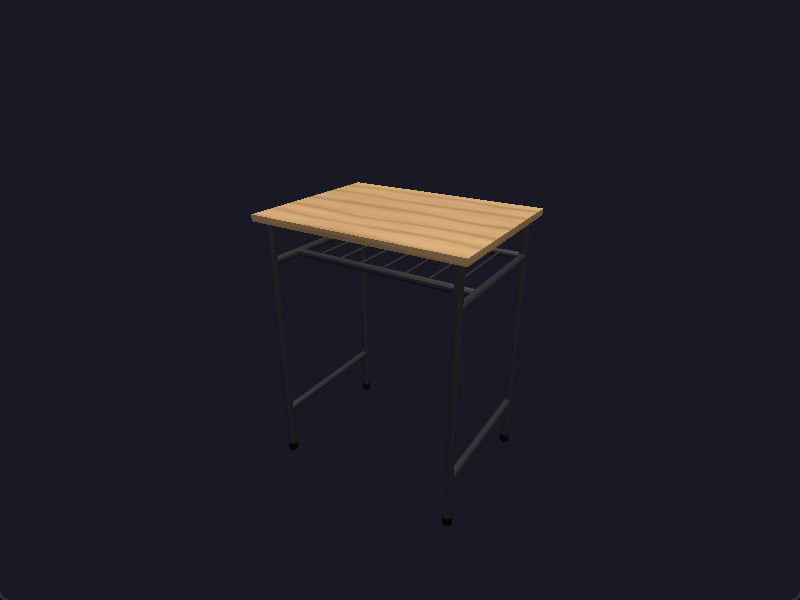
\includegraphics[width=\textwidth]{figuras/inspecao-carteira.png}\caption{Carteira}
  \end{subfigure}\hfill
  \begin{subfigure}{0.32\textwidth}\centering
    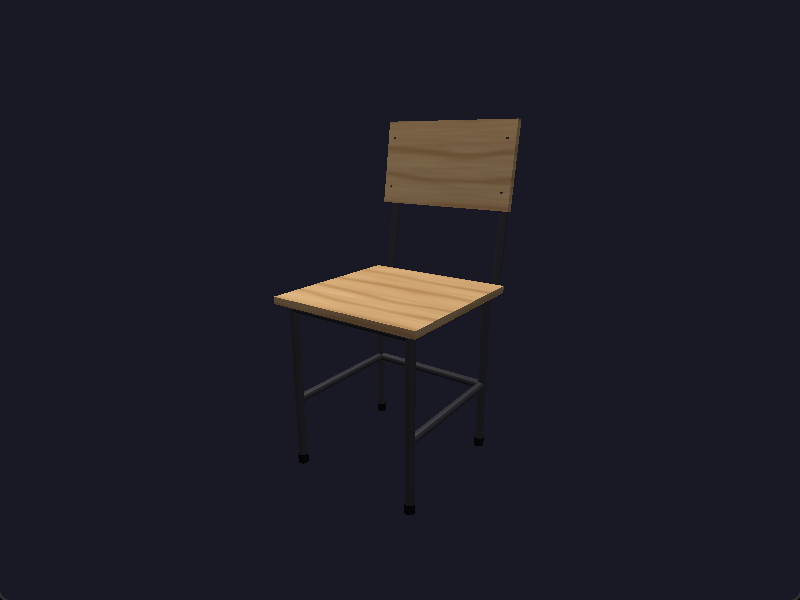
\includegraphics[width=\textwidth]{figuras/inspecao-cadeira.png}\caption{Cadeira}
  \end{subfigure}\hfill
  \begin{subfigure}{0.32\textwidth}\centering
    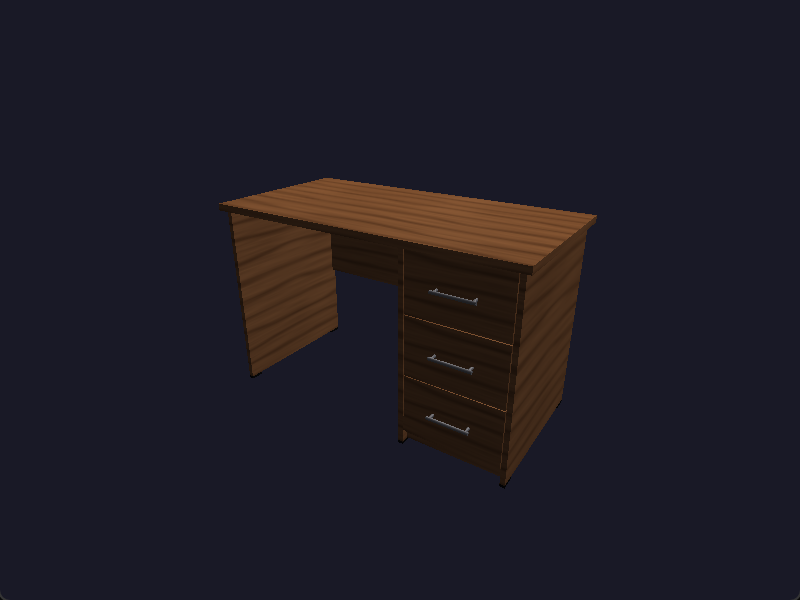
\includegraphics[width=\textwidth]{figuras/inspecao-mesa.png}\caption{Mesa do professor}
  \end{subfigure}

  \medskip
  \begin{subfigure}{0.32\textwidth}\centering
    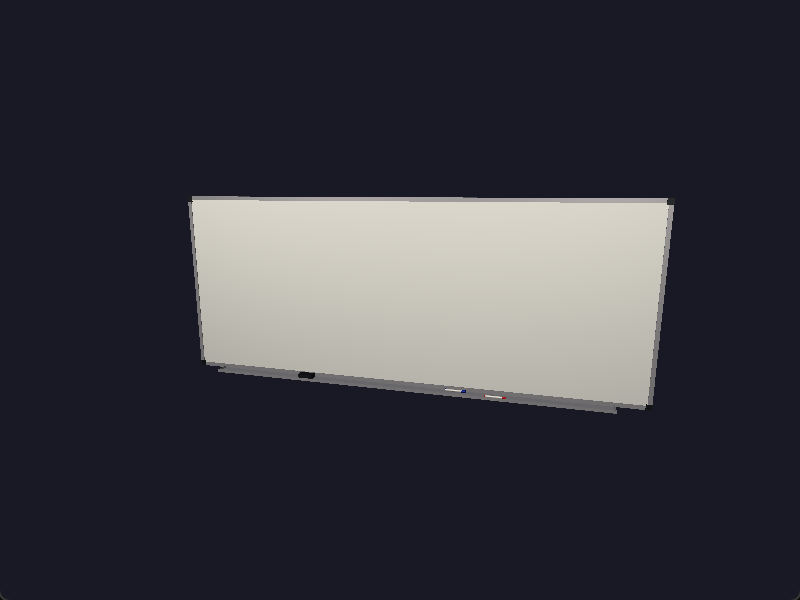
\includegraphics[width=\textwidth]{figuras/inspecao-quadro.png}\caption{Quadro}
  \end{subfigure}\hfill
  \begin{subfigure}{0.32\textwidth}\centering
    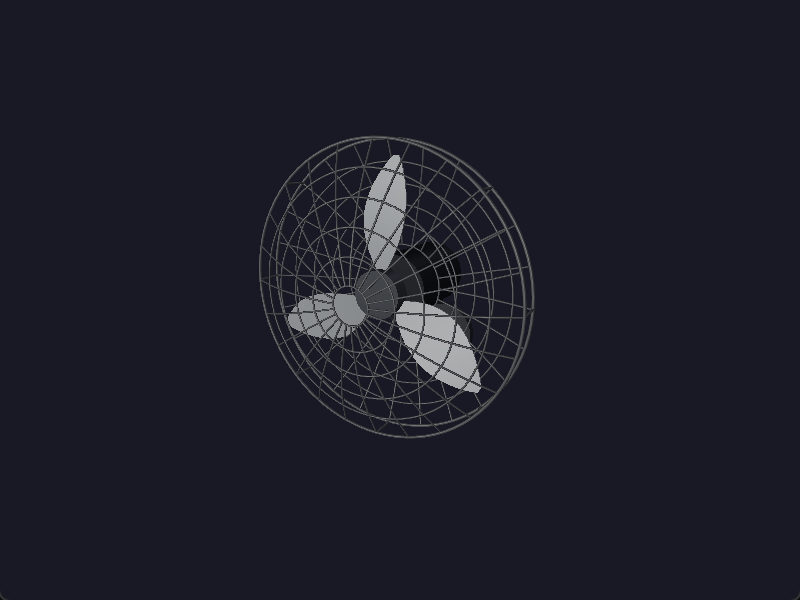
\includegraphics[width=\textwidth]{figuras/inspecao-ventilador.png}\caption{Ventilador}
  \end{subfigure}\hfill
  \begin{subfigure}{0.32\textwidth}\centering
    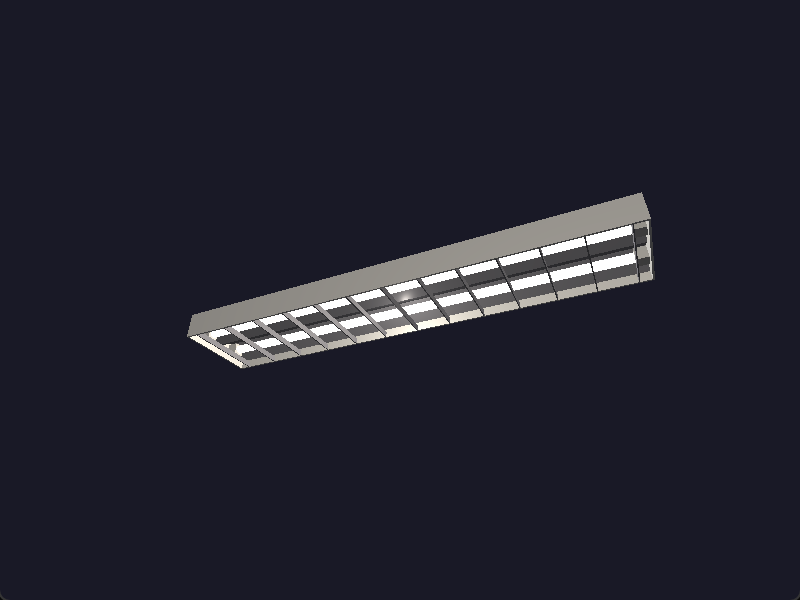
\includegraphics[width=\textwidth]{figuras/inspecao-lampada.png}\caption{Luminária}
  \end{subfigure}

  \medskip
  \begin{subfigure}{0.32\textwidth}\centering
    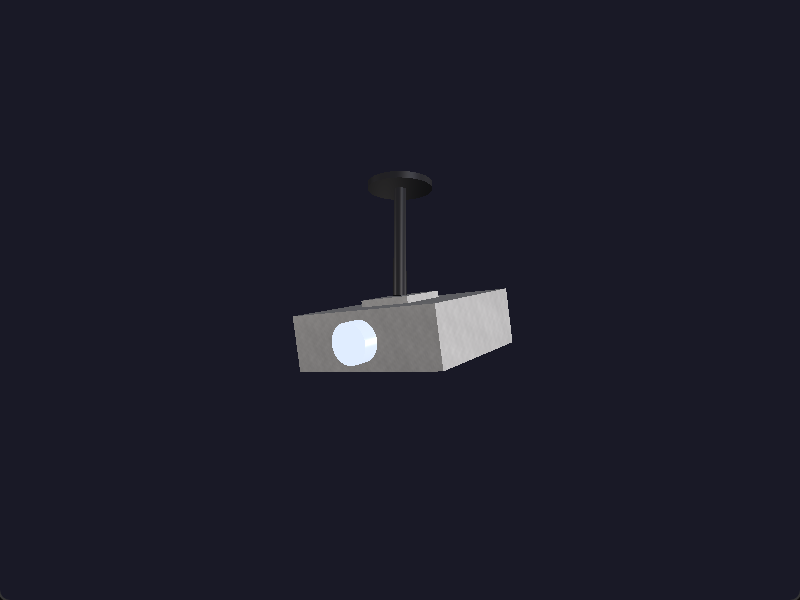
\includegraphics[width=\textwidth]{figuras/inspecao-projetor-ligado.png}\caption{Projetor ligado}
  \end{subfigure}\hfill
  \begin{subfigure}{0.32\textwidth}\centering
    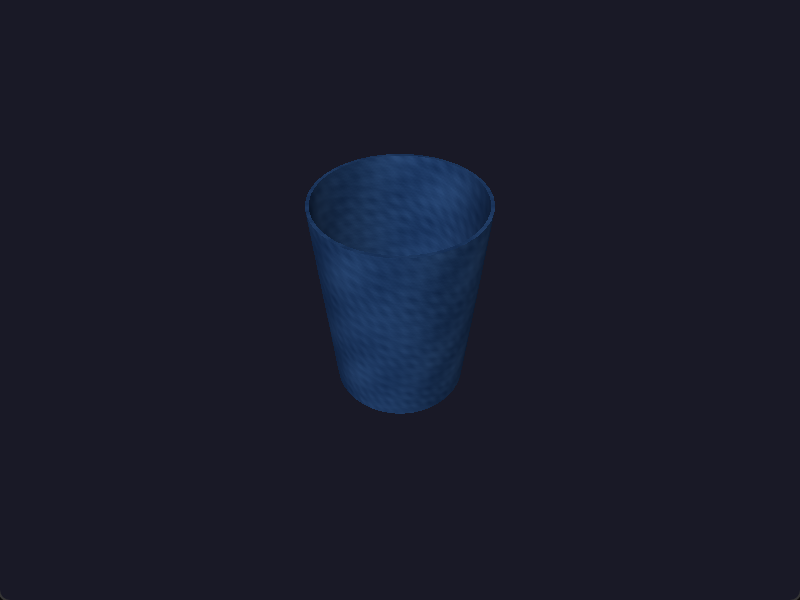
\includegraphics[width=\textwidth]{figuras/inspecao-lixeira.png}\caption{Lixeira}
  \end{subfigure}\hfill
  \begin{subfigure}{0.32\textwidth}\centering
    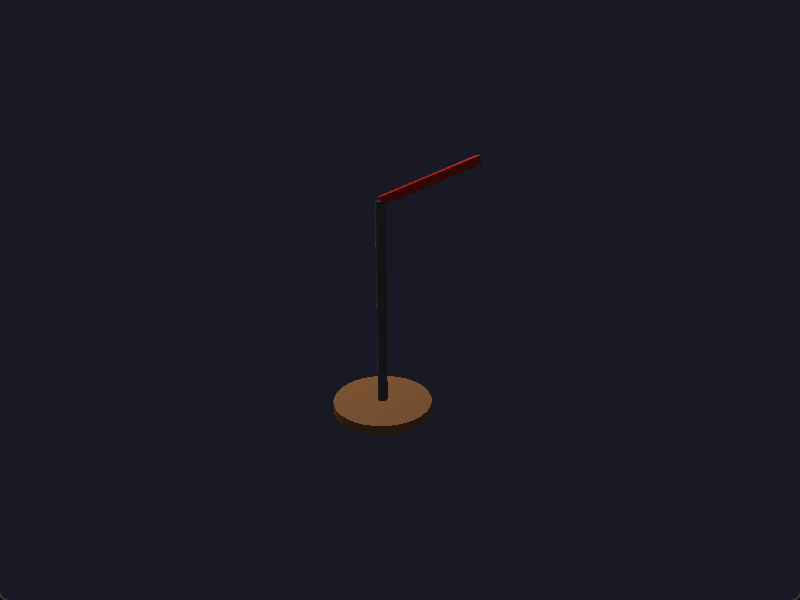
\includegraphics[width=\textwidth]{figuras/inspecao-articulado.png}\caption{Objeto articulado}
  \end{subfigure}
  \fonteautoras
\end{figure}

% -----------------------------------------------------------------------------
\chapter{Transformações geométricas}
\label{cap:transformacoes}

As três transformações usam matrizes 4 × 4 em coordenadas homogêneas \cite{shirley2016}. Um ponto
$\mathbf{p} = (x, y, z, 1)^T$ é transformado por $\mathbf{p}' = M\mathbf{p}$ e, num produto $M = A \cdot B$,
a matriz da direita é aplicada primeiro. As matrizes de translação, escala e rotação em torno de Z são:
\begin{equation}
  T(\mathbf{t}) =
  \begin{bmatrix} 1 & 0 & 0 & t_x \\ 0 & 1 & 0 & t_y \\ 0 & 0 & 1 & t_z \\ 0 & 0 & 0 & 1 \end{bmatrix},\quad
  S(s_x, s_y, s_z) =
  \begin{bmatrix} s_x & 0 & 0 & 0 \\ 0 & s_y & 0 & 0 \\ 0 & 0 & s_z & 0 \\ 0 & 0 & 0 & 1 \end{bmatrix},\quad
  R_z(\theta) =
  \begin{bmatrix} \cos\theta & -\sin\theta & 0 & 0 \\ \sin\theta & \cos\theta & 0 & 0 \\ 0 & 0 & 1 & 0 \\ 0 & 0 & 0 & 1 \end{bmatrix}.
\end{equation}

Escala e rotação acontecem em torno da origem. Para escalar ou girar em torno de um pivô $\mathbf{c}$, o
objeto é modelado com o pivô na origem do nó e a matriz do nó leva essa origem até $\mathbf{c}$:
$T(\mathbf{c}) \cdot X$, com $X$ sendo a escala ou a rotação. Os trechos de código citados a seguir estão
marcados no repositório com o comentário \texttt{AB2~·} e podem ser listados com
\texttt{git grep -n \textquotedbl{}AB2~·\textquotedbl}.

\section{Escala: tela retrátil}

A tela tem uma caixa no alto da parede e uma lona de 2,0 × 1,5 m que desce por uma fenda. A lona é filha de
uma articulação cuja origem é o topo da própria lona: a malha vai de $y = 0$ (topo) a $y = -1{,}5$~m (base).
Para abrir e recolher, só a matriz dessa articulação muda:
\begin{equation}
  M_{\text{lona}} = T(\mathbf{p}_{\text{fenda}}) \cdot S(1,\ s,\ 1), \qquad s \in [0, 1],
  \label{eq:escala}
\end{equation}
em que $s = 0$ é a tela recolhida e $s = 1$, aberta. Lida da direita para a esquerda, a escala em Y acontece em
torno do topo da lona, que é a origem do nó; só depois a translação leva esse topo até a fenda. Um vértice
de altura local $y$ vai para $y_{\text{fenda}} + s \cdot y$: o topo ($y = 0$) não se move e a base sobe
($-1{,}5 s$). A lona encolhe para cima sem descolar da caixa, como uma tela real enrolando no rolo
(\autoref{cod:escala}). A barra inferior não é escalada, só transladada para acompanhar a base:
$T(\mathbf{p}_{\text{fenda}} + (0, -1{,}5 s, 0))$.

\begin{lstlisting}[caption={Escala da lona (\texttt{src/objects/projection\_screen.cpp}, sem comentários)},label={cod:escala}]
void ProjectionScreen::applyOpenAmount() {
    canvasMaterial_.uvScale.y = kCanvasHeight * openAmount_ / kCanvasTexturePeriod;
    if (root_ == nullptr) {
        return;
    }
    canvasPivot_->transform = glm::scale(translated(kSlot), {1.0f, openAmount_, 1.0f});
    canvasPivot_->visible = openAmount_ > kMinVisibleAmount;
    bottom_->transform = translated(kSlot + glm::vec3(0.0f, -kCanvasHeight * openAmount_, 0.0f));
}
\end{lstlisting}
\fonteautores

A tecla \texttt{T} inverte o sentido do movimento. Um progresso $t \in [0, 1]$ avança linearmente com o tempo
(curso completo em 2,5~s) e a escala é suavizada por $s = 3t^2 - 2t^3$ (\emph{smoothstep}), que parte e chega
com velocidade nula. Inverter no meio do curso é contínuo, porque só o sentido de $t$ muda. Dois detalhes
decorrem da escala não uniforme:
\begin{itemize}
  \item \textbf{Textura}: como a escala encurta a lona mas as coordenadas de textura continuam de 0 a 1, a trama
        do tecido achataria em Y. A repetição vertical é ajustada para $1{,}5 s / 0{,}25$, mantendo o período
        de 25~cm;
  \item \textbf{Normais}: a matriz das normais é a inversa transposta (\autoref{sec:normais}); com $s = 0$
        ela não existe (matriz singular), por isso a lona fica invisível abaixo de $s = 0{,}001$.
\end{itemize}

\section{Rotação: ventilador}

O ventilador tem um nó fixo (suporte, motor, eixo e grades) e um nó \emph{rotor} com as três pás e a tampa
central. As pás são modeladas em volta da origem do rotor, que coincide com o eixo do motor (eixo Z local).
A matriz do rotor é
\begin{equation}
  M_{\text{rotor}} = T(\mathbf{c}_{\text{rotor}}) \cdot R_z(\theta),
  \label{eq:rotacao}
\end{equation}
ou seja, gira as pás em torno do eixo e depois as leva ao centro do motor (\autoref{cod:rotacao}). Os vértices
nunca são recalculados: a cada quadro só muda $\theta$. Grades e motor, no nó fixo, não giram.

O ângulo é integrado no tempo pelo método de Euler explícito. Com a velocidade angular $\omega$ (graus por
segundo) e o alvo $\omega^{*}$ ($0$ desligado, ou 720, 1080 ou 1440~°/s, isto é, 2, 3 ou 4 voltas/s):
\begin{align}
  \omega_{k+1} &=
  \begin{cases}
    \min(\omega_k + a_{\uparrow}\,\Delta t,\ \omega^{*}) & \text{se } \omega_k < \omega^{*} \\
    \max(\omega_k - a_{\downarrow}\,\Delta t,\ \omega^{*}) & \text{caso contrário}
  \end{cases} \\
  \theta_{k+1} &= \theta_k + \omega_{k+1}\,\Delta t,
\end{align}
com $a_{\uparrow} = 960$~°/s² (até 1,5~s para atingir a velocidade máxima) e $a_{\downarrow} = 480$~°/s²
(até 3~s para parar). Como tudo é multiplicado por $\Delta t$, o giro por segundo é o mesmo a 30 ou a
144 quadros por segundo. O ângulo é reduzido a $[-180^\circ, 180^\circ]$ a cada passo para não perder precisão no
\texttt{float} depois de horas ligado.

\begin{lstlisting}[caption={Rotação do rotor (\texttt{src/objects/fan.cpp}, sem comentários)},label={cod:rotacao}]
void Fan::setRotorAngle(float degrees) {
    if (!std::isfinite(degrees)) {
        return;
    }
    rotorAngle_ = std::remainder(degrees, 360.0f);
    if (rotor_ != nullptr) {
        rotor_->transform = glm::rotate(translated(kRotorCenter), glm::radians(rotorAngle_), {0, 0, 1});
    }
}

void Fan::update(float deltaTime) {
    const float target = on_ ? kSpeeds[speedLevel_] : 0.0f;
    if (speed_ < target) {
        speed_ = std::min(speed_ + kSpinUp * deltaTime, target);
    } else {
        speed_ = std::max(speed_ - kSpinDown * deltaTime, target);
    }
    if (speed_ > 0.0f) {
        setRotorAngle(rotorAngle_ + speed_ * deltaTime);
    }
}
\end{lstlisting}
\fonteautores

As velocidades ficam bem abaixo das de um ventilador real (cerca de 20 voltas/s) por causa da amostragem
temporal. Com três pás, o rotor é simétrico a cada 120°; se o giro entre dois quadros passar de 60°, o olho
associa cada pá à pá vizinha e o rotor parece girar devagar, parado ou para trás (efeito ``roda de carroça'').
A 4 voltas/s e 60 quadros por segundo, o passo é de 24° por quadro; mesmo a 30 quadros por segundo, de 48°.
A 20 voltas/s seriam 120° por quadro, e as pás pareceriam paradas.

\section{Projeção: slide do projetor}
\label{sec:projecao}

O slide não é uma textura colada na lona. O projetor é tratado como uma luz que carrega uma imagem, pela
técnica de textura projetiva \cite{segal1992}: cada fragmento da cena descobre em que ponto da imagem do
projetor ele está e recebe a luz daquele texel. A imagem cai onde o feixe bater: na lona aberta, ou no quadro e
na parede com a tela recolhida.

A pergunta ``onde este ponto cai na imagem?'' é a mesma que a câmera responde ao desenhar a cena. Por isso o
projetor ganha uma matriz de visualização e uma de projeção próprias, como uma câmera posta na lente:
\begin{align}
  V_{\text{proj}} &= \mathrm{lookAt}(\mathbf{l},\ \mathbf{l} + \mathbf{d},\ \mathbf{u}), \\
  P_{\text{proj}} &= \mathrm{perspective}(\mathit{fov}_y,\ 4/3,\ 0{,}1~\text{m},\ 10~\text{m}),
\end{align}
em que $\mathbf{l}$, $\mathbf{d}$ e $\mathbf{u}$ são o centro, o eixo e o ``cima'' da lente levados ao mundo.
O produto $P_{\text{proj}} V_{\text{proj}}$ é calculado uma vez, na CPU (\autoref{cod:projecao-cpu}), e
enviado ao fragment shader, onde cada fragmento de posição $\mathbf{p}$ percorre a cadeia
\begin{equation}
  \mathbf{c} = P_{\text{proj}} V_{\text{proj}} \begin{bmatrix}\mathbf{p}\\1\end{bmatrix}, \qquad
  \mathbf{n} = \frac{(c_x, c_y, c_z)}{c_w} \in [-1, 1]^3, \qquad
  (u, v) = 0{,}5\,(n_x, n_y) + 0{,}5 \in [0, 1]^2 .
  \label{eq:projecao}
\end{equation}
A divisão por $c_w$ é a divisão de perspectiva que a GPU faz sozinha com \texttt{gl\_Position}; aqui ela é
feita à mão. Fragmentos com $c_w \le 0$ (atrás da lente) ou com $\mathbf{n}$ fora do cubo $[-1, 1]^3$ (fora
da imagem, antes do plano próximo ou depois do distante) não recebem luz (\autoref{cod:projecao-gpu}).

O ângulo de abertura vem da geometria real. A lente fica a $d = 2{,}89$~m do centro da lona e a imagem
ocupa $w = 1{,}84$~m de largura (92\% dos 2,0~m da lona):
\begin{equation}
  \mathit{fov}_x = 2\arctan\frac{w/2}{d} = 2\arctan\frac{0{,}92}{2{,}89} \approx 35{,}3^\circ, \qquad
  \mathit{fov}_y = 2\arctan\frac{\tan(\mathit{fov}_x/2)}{4/3} \approx 26{,}9^\circ.
\end{equation}
Como o projetor está acima do centro da lona e inclinado para baixo, a borda inferior da imagem fica mais longe
da lente (cerca de 3,05~m) que a superior (2,73~m) e sai mais larga: a imagem forma um trapézio
(\emph{keystone}), como num projetor real sem correção. A margem de 8\% evita que a base passe da lona.

\begin{lstlisting}[caption={Matrizes do projetor (\texttt{src/scene/classroom.cpp}, sem comentários)},label={cod:projecao-cpu}]
const glm::vec3 lensPosition = toWorld(projectorPlacement, projector_.lensCenter());
const glm::mat3 projectorRotation(projectorPlacement);
const glm::vec3 lensDirection = glm::normalize(projectorRotation * projector_.lensDirection());
const glm::vec3 lensUp = glm::normalize(projectorRotation * projector_.lensUp());
const float throwDistance = glm::distance(lensPosition, screenCenter);
const float halfImageWidth = kImageFill * screen_.canvasSize().x * 0.5f;
const float fovX = 2.0f * std::atan(halfImageWidth / throwDistance);
const float fovY = 2.0f * std::atan(std::tan(fovX * 0.5f) / kSlideAspect);
const glm::mat4 projectorView = glm::lookAt(lensPosition, lensPosition + lensDirection, lensUp);
const glm::mat4 projectorProjection = glm::perspective(fovY, kSlideAspect, kProjectorNear, kProjectorFar);
lighting_.projector.viewProjection = projectorProjection * projectorView;
\end{lstlisting}
\fonteautores

\begin{lstlisting}[language=GLSL,caption={Luz do projetor no fragmento (\texttt{shaders/basic.frag}, sem comentários)},label={cod:projecao-gpu}]
vec3 projectorLight(vec3 N, vec3 albedo) {
    if (!uProjector.enabled) {
        return vec3(0.0);
    }
    vec4 clip = uProjector.viewProjection * vec4(vWorldPos, 1.0);
    if (clip.w <= 0.0) {
        return vec3(0.0);
    }
    vec3 ndc = clip.xyz / clip.w;
    if (any(lessThan(ndc, vec3(-1.0))) || any(greaterThan(ndc, vec3(1.0)))) {
        return vec3(0.0);
    }
    vec2 uv = ndc.xy * 0.5 + 0.5;
    vec3 toLens = uProjector.position - vWorldPos;
    float d = max(length(toLens), kEpsilon);
    float lambert = max(dot(N, toLens / d), 0.0);
    float falloff = (uProjector.referenceDistance * uProjector.referenceDistance) / (d * d);
    return albedo * texture(uProjector.image, uv).rgb * uProjector.color * lambert * falloff;
}
\end{lstlisting}
\fonteautores

A contribuição do projetor é somada às outras luzes:
\begin{equation}
  L_{\text{proj}} = \mathbf{a} \odot \mathrm{slide}(u, v) \odot \mathbf{c}_{\text{proj}} \cdot
  \max(\mathbf{N}\cdot\mathbf{L}, 0) \cdot \left(\frac{d_{\text{ref}}}{d}\right)^2,
\end{equation}
em que $\mathbf{a}$ é a cor difusa da superfície, $d$ a distância até a lente e $d_{\text{ref}}$ a distância
até o centro da lona, onde o fator vale 1. As partes brancas do slide iluminam; as pretas não projetam nada
e a superfície fica com a cor que a sala já lhe dá. A orientação foi conferida pelo bloco laranja no canto
superior esquerdo de cada slide: a imagem aparece em pé e sem espelhamento (\autoref{fig:projetor}).

\begin{figure}[htb]
  \centering
  \caption{Projeção do slide na tela retrátil}
  \label{fig:projetor}
  \begin{subfigure}{0.49\textwidth}\centering
    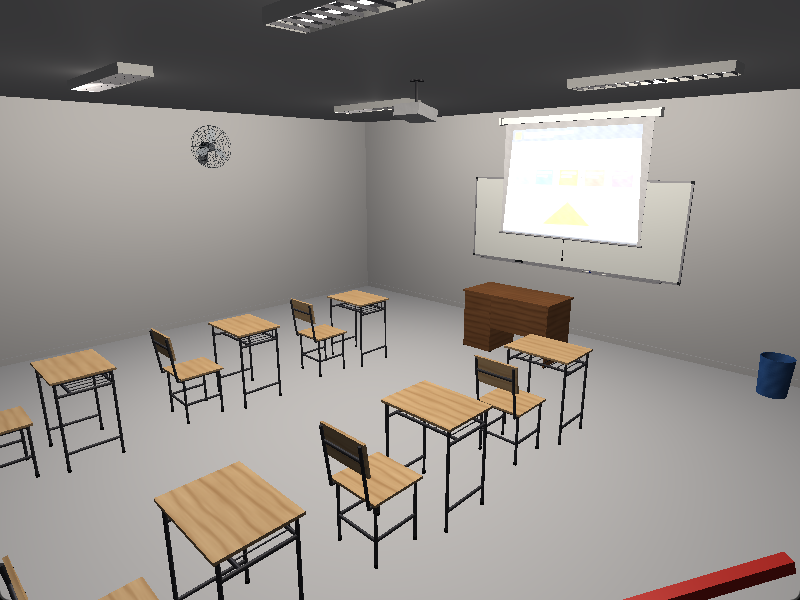
\includegraphics[width=\textwidth]{figuras/projetor-ligado.png}
    \caption{Luzes acesas: pouco contraste}
  \end{subfigure}\hfill
  \begin{subfigure}{0.49\textwidth}\centering
    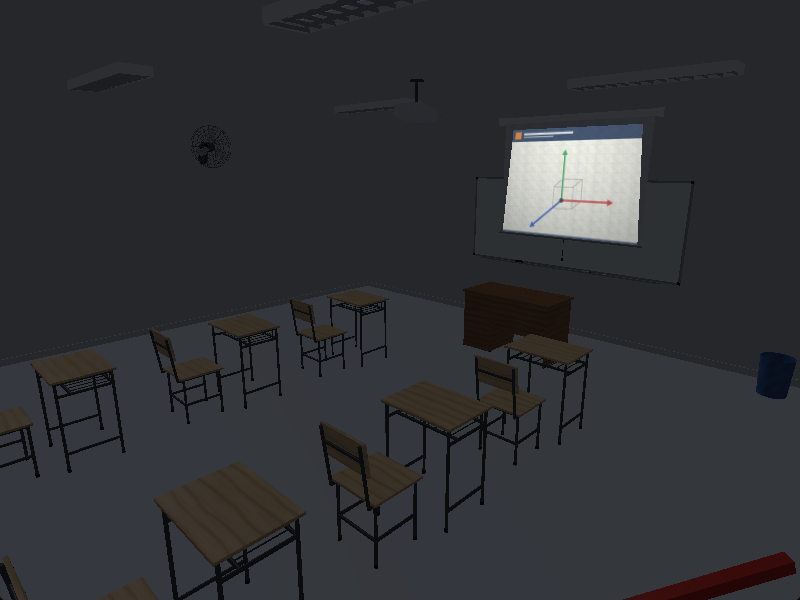
\includegraphics[width=\textwidth]{figuras/luzes-apagadas.png}
    \caption{Luzes apagadas, segundo slide}
  \end{subfigure}
  \fonteautoras
\end{figure}

A principal limitação é a ausência de \emph{shadow mapping}: o shader não sabe se há algo entre a lente e o
fragmento. A imagem também chega ao quadro atrás da lona aberta (escondida pela própria lona para quem está na
sala), e um objeto à frente do projetor recebe a imagem sem fazer sombra na tela.

% -----------------------------------------------------------------------------
\chapter{Iluminação, materiais e texturas}
\label{cap:iluminacao}

\section{Modelo de Blinn-Phong}

A cor é calculada por fragmento no fragment shader, com o modelo de Blinn-Phong \cite{phong1975,blinn1977}.
Com $\mathbf{N}$ a normal, $\mathbf{L}$ a direção para a luz, $\mathbf{V}$ a direção para a câmera e
$\mathbf{H} = \mathrm{normalize}(\mathbf{L} + \mathbf{V})$, todos unitários:
\begin{equation}
  \mathbf{cor} = \mathbf{e} + \mathbf{a}_{\text{amb}} \odot \mathbf{a}
  + \sum_i f_i\, \mathbf{c}_i \odot \left[ \max(\mathbf{N}\cdot\mathbf{L}_i, 0)\, \mathbf{a}
  + \max(\mathbf{N}\cdot\mathbf{H}_i, 0)^{\alpha}\, \mathbf{k}_s \right] + L_{\text{proj}},
\end{equation}
em que $\mathbf{e}$ é a cor emissiva, $\mathbf{a}$ a difusa (albedo), $\mathbf{k}_s$ a especular, $\alpha$ o
brilho, $\mathbf{c}_i$ a cor da luz e $f_i$ a atenuação. O termo especular é zerado quando
$\mathbf{N}\cdot\mathbf{L} \le 0$, e os vetores que podem ser nulos são protegidos por um $\varepsilon = 10^{-4}$.
O Blinn-Phong foi preferido ao Phong original porque o reflexo enfraquece suavemente em ângulos abertos, sem a
borda que $\mathbf{R}\cdot\mathbf{V}$ produz ao ficar negativo, e porque é mais barato
\cite{akenine2018}.

A sala tem quatro luzes pontuais, uma por luminária, com atenuação
\begin{equation}
  f(d) = \frac{1}{k_c + k_l d + k_q d^2}, \qquad k_c = 1,\ k_l = 0{,}14,\ k_q = 0{,}07,
\end{equation}
além de uma luz ambiente constante e de uma luz direcional fraca vinda da esquerda (-X), que representa a
claridade do dia e dá volume às faces que as lâmpadas iluminam de lado. A tecla \texttt{L} desliga as luzes
pontuais, apaga a emissiva dos tubos e reduz a luz ambiente; a sala escurece, mas não fica preta
(\autoref{fig:projetor}).

\section{Matriz das normais}
\label{sec:normais}

As normais não podem ser transformadas pela mesma matriz dos vértices quando há escala não uniforme, como na
lona. Uma normal $\mathbf{n}$ precisa continuar perpendicular a qualquer tangente $\mathbf{t}$ depois da
transformação. Se $\mathbf{t}' = M\mathbf{t}$, procura-se $G$ tal que
$(G\mathbf{n})^T (M\mathbf{t}) = \mathbf{n}^T (G^T M)\, \mathbf{t} = 0$ para todo $\mathbf{t}$ com
$\mathbf{n}^T\mathbf{t} = 0$, o que vale com $G^T M = I$:
\begin{equation}
  G = \left(M_{3\times3}^{-1}\right)^T .
\end{equation}
A matriz é calculada na CPU, uma vez por peça (\autoref{cod:scenenode}), e não no vertex shader, uma vez por
vértice.

\section{Materiais e texturas}

Cada peça tem um material com cor difusa, textura opcional e sua escala de repetição, cor especular, brilho e
cor emissiva. Há predefinições para metal, madeira, plástico e superfícies foscas, e o material é herdado
pela árvore: vai na raiz do objeto e só as peças diferentes o sobrescrevem. As texturas (laminado das
carteiras e cadeiras, madeira da mesa do professor, trama da lona, plásticos do projetor e da lixeira e os três
slides) são PNGs carregados com stb\_image, com \emph{mipmaps}; as coordenadas de textura das primitivas são
geradas em metros, então a mesma imagem tem a mesma escala em peças de tamanhos diferentes.

% -----------------------------------------------------------------------------
\chapter{Câmera e interação}
\label{cap:camera}

A câmera livre guarda posição e dois ângulos: guinada (\emph{yaw}, $\psi$) e arfagem (\emph{pitch}, $\phi$).
A direção de visão é
\begin{equation}
  \mathbf{f} = (\cos\psi\cos\phi,\ \sin\phi,\ \sin\psi\cos\phi),
\end{equation}
e a matriz de visualização é $\mathrm{lookAt}(\mathbf{p}, \mathbf{p} + \mathbf{f}, \hat{\mathbf{y}})$. A
projeção é perspectiva, com 60° de abertura vertical, plano próximo a 0,1~m e distante a 100~m
\cite{devries2020}. O mouse altera os ângulos a 0,1° por pixel, e a arfagem fica limitada a ±89°: em 90°,
$\mathbf{f}$ ficaria paralelo ao vetor ``cima'' e o \texttt{lookAt} não teria como definir a direita. As teclas
\texttt{W}, \texttt{A}, \texttt{S} e \texttt{D} movem a câmera a 2~m/s no plano da visão e \texttt{Espaço} e
\texttt{Ctrl} a sobem e descem; o deslocamento combinado é normalizado, para a diagonal não ser mais rápida.

O clique esquerdo captura o cursor; com ele livre, não há movimento, mas a inspeção e as interações continuam
funcionando. As teclas \texttt{1} a \texttt{0} e \texttt{[}/\texttt{]} selecionam a cena completa ou um dos
onze alvos de inspeção. As interações são tratadas em \texttt{Classroom::update}, que chama o método do objeto:
\texttt{L} (luzes), \texttt{T} (tela), \texttt{V} e \texttt{Shift}+\texttt{V} (ventilador), \texttt{P} e as
setas (projetor). A lista completa está no Apêndice~\ref{ap:comandos}.

% -----------------------------------------------------------------------------
\chapter{Resultados}
\label{cap:resultados}

A sala roda em tempo real em placas de vídeo integradas e também por renderização em software (Mesa
llvmpipe). A \autoref{fig:tela} mostra a tela retrátil aberta pela tecla \texttt{T}, antes de o projetor ser
ligado; a \autoref{fig:projetor}, o slide projetado com as luzes acesas e apagadas. Todas as figuras deste
relatório foram capturadas do programa compilado a partir de um clone limpo do repositório.

\begin{figure}[htb]
  \centering
  \caption{Tela retrátil aberta, com o projetor desligado}
  \label{fig:tela}
  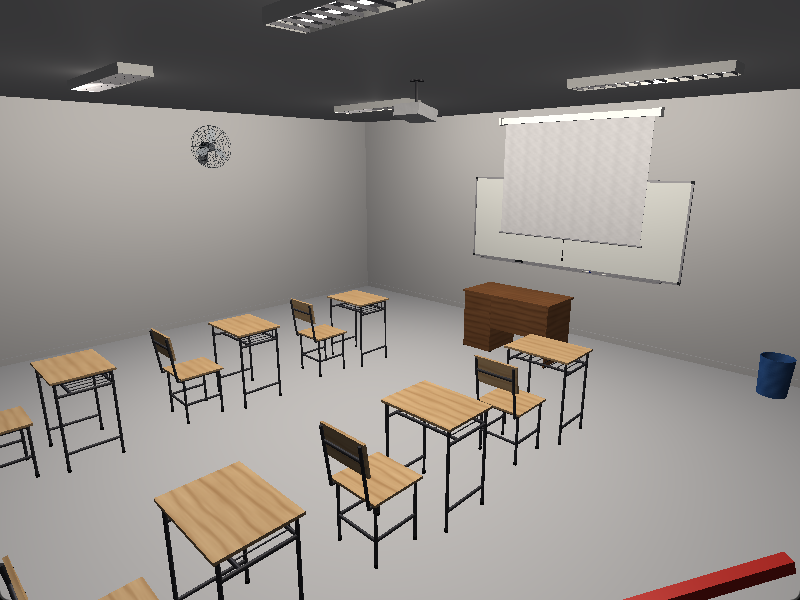
\includegraphics[width=0.75\textwidth]{figuras/tela-aberta.png}
  \fonteautoras
\end{figure}

Os requisitos da avaliação foram atendidos: objetos modelados pela equipe, iluminação com materiais e
texturas, câmera navegável, inspeção de cada objeto e as três transformações ligadas a interações. O programa
compila sem avisos com \texttt{-Wall -Wextra -Wpedantic}.

% -----------------------------------------------------------------------------
\chapter{Compilação e execução}
\label{cap:compilacao}

O passo a passo completo está no README do repositório. Em resumo, do sistema vêm só o compilador, o CMake,
o Git e, no Linux, os headers do X11; as bibliotecas são compiladas a partir de \texttt{lib/}. No Windows, com o
g++ do MSYS2 (UCRT64) no \texttt{Path}:

\begin{lstlisting}[language=bash,caption={Compilação no Windows (PowerShell)},label={cod:build-windows}]
git clone https://github.com/JoseRiquelmeTds/ambiente-sala-de-aula-opengl.git
cd ambiente-sala-de-aula-opengl
cmake --preset windows
cmake --build --preset windows --target run
\end{lstlisting}
\fonteautores

No Linux (Ubuntu) e no WSL2:

\begin{lstlisting}[language=bash,caption={Compilação no Linux},label={cod:build-linux}]
sudo apt install -y git build-essential cmake libx11-dev libxrandr-dev \
  libxinerama-dev libxcursor-dev libxi-dev mesa-utils
git clone https://github.com/JoseRiquelmeTds/ambiente-sala-de-aula-opengl.git
cd ambiente-sala-de-aula-opengl
cmake --preset linux
cmake --build --preset linux --target run
\end{lstlisting}
\fonteautores

O build limpo da versão final (tag \texttt{v1.0.0}) foi testado com um clone novo, seguindo só o README, nos
sistemas do \autoref{tab:sistemas}.

\begin{table}[htb]
  \centering
  \caption{Sistemas testados}
  \label{tab:sistemas}
  \footnotesize
  \begin{tabularx}{\textwidth}{|X|l|l|X|}
    \hline
    \textbf{Sistema} & \textbf{Compilador} & \textbf{CMake} & \textbf{Vídeo} \\
    \hline
    Windows 11 Pro & g++ 16.2.0 (MSYS2) & 4.4.2 & Intel Graphics (OpenGL 3.3) \\
    Ubuntu 24.04.5 LTS (contêiner limpo) & g++ 13.3.0 & 3.28.3 & Mesa 25.2.8, llvmpipe (OpenGL 4.5) \\
    Ubuntu 26.04.1 LTS (contêiner limpo) & g++ 15.2.0 & 4.2.3 & Mesa 26.0.8, llvmpipe (OpenGL 4.5) \\
    \hline
  \end{tabularx}
  \fonteautores
\end{table}

% -----------------------------------------------------------------------------
\chapter{Divisão de tarefas}
\label{cap:equipe}

O trabalho foi organizado em tarefas (cards CG-$n$) num quadro Jira, com uma branch e um \emph{pull request}
revisado por outro integrante para cada tarefa. O \autoref{tab:equipe} resume as responsabilidades.

\begin{table}[htb]
  \centering
  \caption{Responsabilidades por integrante}
  \label{tab:equipe}
  \footnotesize
  \begin{tabularx}{\textwidth}{|l|X|}
    \hline
    \textbf{Integrante} & \textbf{Tarefas} \\
    \hline
    Erasmo da Silva Sá Junior & Build com CMake e bibliotecas embutidas; convenções e arquitetura (CG-53,
      CG-87); projetor, tela retrátil e lixeira (CG-65 a CG-67); escala da tela (CG-75), rotação do
      ventilador (CG-76) e projeção do slide (CG-77); texturas da tela, do projetor e da lixeira (CG-78);
      entrega final (CG-81) \\
    José Riquelme Teixeira da Silva & Malha, primitivas, shader e carregador de texturas (CG-56 a CG-58);
      carteira, luminária com interruptor e mesa do professor (CG-62 a CG-64); iluminação Blinn-Phong
      (CG-71), materiais por peça (CG-72), interação da luz (CG-73) e texturas desses objetos (CG-74) \\
    Victor André Lopes Brasileiro & Janela, entrada e loop (CG-54); câmera livre e inspeção (CG-55);
      ventilador, cadeira e quadro (CG-59 a CG-61); montagem da sala (CG-69); materiais da cadeira, do
      ventilador e do quadro (CG-74); revisão da navegação (CG-68) \\
    \hline
  \end{tabularx}
  \fonteautores
\end{table}

% -----------------------------------------------------------------------------
\chapter{Conclusão}
\label{cap:conclusao}

O projeto entregou uma sala de aula navegável e interativa usando apenas o pipeline programável do OpenGL 3.3.
A organização em grafo de cena foi o ponto central: as três transformações da avaliação se reduzem a trocar a
matriz de um único nó articulado (\autoref{eq:escala}, \autoref{eq:rotacao}) ou a tratar o projetor como uma
câmera (\autoref{eq:projecao}), sem reconstruir geometria. A escala não uniforme da lona mostrou na prática por
que as normais exigem a inversa transposta, e a rotação do ventilador mostrou o efeito da amostragem temporal na
escolha das velocidades.

Ficam como limitações e trabalhos futuros a ausência de sombras (\emph{shadow mapping}), que também
impediria a imagem do projetor de atravessar a lona, a ausência de colisão da câmera com os objetos e a
iluminação apenas local, sem luz rebatida.

% =============================================================================
%  Elementos pós-textuais
% =============================================================================
\postextual

\printbibliography[title={Referências}]

\begin{apendicesenv}

\chapter{Lista de comandos}
\label{ap:comandos}

Teclado e mouse com a janela em foco. As teclas são identificadas pela posição no teclado americano, como faz
o GLFW; no teclado ABNT2, \texttt{[} e \texttt{]} são as duas teclas à direita do \texttt{P} (as que têm
\texttt{´} e \texttt{[}), e não o \texttt{]} perto do Enter.

\begin{table}[htb]
  \centering
  \caption{Comandos do programa}
  \label{tab:comandos}
  \footnotesize
  \begin{tabularx}{\textwidth}{|l|X|}
    \hline
    \textbf{Controle} & \textbf{Ação} \\
    \hline
    \multicolumn{2}{|l|}{\textit{Janela e cursor}} \\
    Clique esquerdo & Captura o cursor e ativa a navegação \\
    \texttt{Esc} & Libera o cursor; com o cursor já livre, fecha o programa \\
    \texttt{Q} & Fecha o programa \\
    \multicolumn{2}{|l|}{\textit{Navegação (cursor capturado)}} \\
    Mouse & Olha para os lados e para cima/baixo (arfagem limitada a ±89°) \\
    \texttt{W} / \texttt{S} & Avança / recua na direção da câmera \\
    \texttt{A} / \texttt{D} & Move para a esquerda / direita \\
    \texttt{Espaço} / \texttt{Ctrl} esquerdo & Sobe / desce \\
    \multicolumn{2}{|l|}{\textit{Inspeção}} \\
    \texttt{1} & Cena completa \\
    \texttt{2} a \texttt{9}, \texttt{0} & Carteira, objeto articulado, ventilador, luminária, interruptor, mesa
      do professor, tela retrátil, projetor e lixeira \\
    \texttt{[} / \texttt{]} & Alvo anterior / próximo, em ciclo pelos onze alvos (inclui cadeira e quadro) \\
    \multicolumn{2}{|l|}{\textit{Interações}} \\
    \texttt{L} & Liga / desliga as luzes do teto (a tecla do interruptor bascula junto) \\
    \texttt{T} & Abre / recolhe a tela retrátil (escala) \\
    \texttt{V} & Liga / desliga o ventilador (rotação) \\
    \texttt{Shift} + \texttt{V} & Troca a velocidade do ventilador: 2, 3 ou 4 voltas/s \\
    \texttt{P} & Liga / desliga o projetor (projeção) \\
    $\leftarrow$ / $\rightarrow$ & Slide anterior / próximo \\
    \hline
  \end{tabularx}
  \fonteautores
\end{table}

\end{apendicesenv}

\end{document}
